% ============================================================
% FINAL PROJECT REPORT - ENGLISH VERSION
% Project 11: Fake News & Misinformation Detection System
% Course: CSC15012 - Applications of NLP in Industry
% Student: Le Dinh Minh Quan - 23127460 - 23CNTThuc
% ============================================================
\documentclass[12pt,a4paper]{article}

\usepackage[utf8]{inputenc}
\usepackage{geometry}
\geometry{left=2.3cm, right=2.3cm, top=2.5cm, bottom=2.5cm}
\usepackage{setspace}
\setstretch{1.25}
\usepackage{graphicx}
\usepackage{float}
\usepackage{booktabs}
\usepackage{longtable}
\usepackage{tabularx}
\usepackage{array}
\usepackage{hyperref}
\hypersetup{colorlinks=true, linkcolor=blue, urlcolor=blue, citecolor=blue, breaklinks=true}
\usepackage{xurl}
\usepackage{seqsplit}
\usepackage{listings}
\usepackage{xcolor}
\usepackage{amsmath}
\usepackage{caption}
\usepackage{subcaption}
\usepackage{enumitem}
\usepackage{fancyhdr}
\usepackage{tikz}
\usetikzlibrary{shapes.geometric, arrows.meta, positioning, fit, backgrounds, shadows}

% --- Make long inline code / paths break gracefully ---
\sloppy
\tolerance=2000
\emergencystretch=3em
\hbadness=10000
\setlength{\parskip}{0.15em}

% Helper for breakable monospaced paths
\newcommand{\bpath}[1]{\seqsplit{#1}}
\newcommand{\btt}[1]{\texttt{\seqsplit{#1}}}

% New column type for tabularx: left-aligned and ragged-right with breaking
\newcolumntype{L}{>{\raggedright\arraybackslash}X}

\lstset{
  basicstyle=\ttfamily\small,
  breaklines=true,
  frame=single,
  backgroundcolor=\color{gray!10},
  keywordstyle=\color{blue},
  commentstyle=\color{green!60!black},
  stringstyle=\color{red!70!black},
  showstringspaces=false,
  tabsize=2
}

\pagestyle{fancy}
\fancyhf{}
\fancyhead[L]{\small CSC15012 -- Final Project Report}
\fancyhead[R]{\small Le Dinh Minh Quan -- 23127460}
\fancyfoot[C]{\thepage}

% ============================================================
\begin{document}

% --- TITLE PAGE ---
\begin{titlepage}
\centering
\vspace*{0.5cm}

% HCMUS LOGO: upload logo_hcmus.png to Overleaf and the next line shows it (absent = no error)
\IfFileExists{logo_hcmus.png}{\includegraphics[width=3.5cm]{logo_hcmus.png}\\[0.5cm]}{}

{\large \textbf{VIETNAM NATIONAL UNIVERSITY HO CHI MINH CITY}}\\[0.3cm]
{\Large \textbf{UNIVERSITY OF SCIENCE}}\\[0.3cm]
{\large Faculty of Information Technology}\\[1.5cm]

{\LARGE \textbf{FINAL PROJECT REPORT}}\\[0.5cm]
{\large Course: \textbf{CSC15012 -- Applications of Natural Language\\ Processing in Industry}}\\[1.5cm]

{\Large \textbf{Project 11:}}\\[0.3cm]
{\Large \textbf{Fake News and Misinformation Detection}}\\[0.3cm]
{\large A Trainable Credibility Classifier wrapped by an\\ Agentic, Evidence-Grounded Fact-Check}\\[2cm]

\begin{tabular}{ll}
\textbf{Student:} & Le Dinh Minh Quan \\
\textbf{Student ID:} & 23127460 \\
\textbf{Class:} & 23CNTThuc \\
\end{tabular}

\vfill
{\large Ho Chi Minh City, 2026}
\end{titlepage}

\tableofcontents
\newpage

% ============================================================
\section{Introduction}
% ============================================================

The volume of online news, posts and claims now far exceeds the capacity of professional fact-checkers and platform moderators. Misinformation spreads faster than human review can keep up, yet the wrong automated response -- silently removing or blocking content -- threatens free speech and silences legitimate journalism. The hard part is not just \emph{detecting} suspicious content, but doing so \textbf{transparently}, with cited evidence, and \textbf{never} taking an irreversible action automatically.

This project implements a complete \textbf{Fake News \& Misinformation Detection System} end-to-end. It combines two clearly separated signals:

\begin{itemize}
  \item A \textbf{trainable transformer classifier} (with a TF-IDF + Logistic Regression baseline) that produces a fast credibility \emph{prior} $P(\text{fake})$ -- a style/source signal, explicitly \emph{not} a verdict.
  \item An \textbf{agentic, evidence-grounded fact-check}: a deterministic finite-state machine (FSM) that extracts the central claim, retrieves evidence, judges per-evidence stance with NLI, aggregates a verdict with verbatim citations, and \textbf{abstains} (\texttt{unverified}) when the evidence is insufficient.
\end{itemize}

\textbf{Non-negotiable framing.} The system \emph{flags content for human review and always shows its evidence -- it never auto-removes, auto-blocks, or auto-censors.} \texttt{unverified} (abstain) is a first-class outcome, not a failure mode. The classifier \emph{prior} and the evidence \emph{verdict} are reported \textbf{separately} so a reviewer always sees when they disagree. This is an \emph{assistant} to human fact-checkers, not an automated arbiter of truth.

\textbf{Project Resources (public):}
\begin{itemize}\setlength\itemsep{0.15em}
  \item \textbf{GitHub repository (source code):} \url{https://github.com/ledinhminhquan/11_Fake_News_Detection}
  \item \textbf{Reference dataset/crawler:} KaiDMML/FakeNewsNet -- \url{https://github.com/KaiDMML/FakeNewsNet}
  \item \textbf{Deployable surfaces (in-repo):} FastAPI REST service (\texttt{/classify} + \texttt{/factcheck}), Gradio demo UI, \texttt{fakenews} CLI, Docker image / Hugging Face Space, and a one-button Colab H100 autopilot notebook.
\end{itemize}

\textit{Deployment status:} the system is fully deployable (API + UI + Docker + Colab autopilot) but is not currently hosted at a fixed public live URL; this report describes the delivered deployment \emph{capability}.

% ============================================================
\section{Business Problem Definition}
% ============================================================

\subsection{Context and Motivation}

Newsrooms, fact-checking organisations and platform trust-\&-safety teams face:
\begin{itemize}
  \item \textbf{Volume vs.\ capacity}: a firehose of posts and claims far exceeds the number of human reviewers; clearly-credible items waste scarce reviewer attention.
  \item \textbf{Cost of the wrong error}: flagging \emph{legitimate} journalism as fake (a false positive) chills lawful speech -- the single most expensive error in this domain.
  \item \textbf{Trust \& accountability}: any credibility signal must be auditable; a verdict without evidence is not actionable and is dangerous if wired to enforcement.
\end{itemize}

\subsection{Target Users and Stakeholders}

\begin{table}[H]
\centering
\caption{Users and jobs-to-be-done}
\small
\begin{tabularx}{\linewidth}{@{} l L L @{}}
\toprule
\textbf{User} & \textbf{Job-to-be-done} & \textbf{What the system gives them} \\
\midrule
Journalists / professional fact-checkers & ``Is this claim worth checking, and what does the evidence say?'' & A verdict (\texttt{real}/\texttt{fake}/\texttt{unverified}) with cited evidence and a line-by-line audit trace \\
Platform trust-\&-safety / moderators & Triage a firehose of posts (flag-for-review) & A fast credibility prior that routes only suspicious items to humans -- never an auto-takedown \\
Newsroom editors / researchers & Rate source/claim credibility on a scale & A 6-way LIAR-style credibility score (pants-fire $\rightarrow$ true) for nuance beyond binary \\
End readers (secondary) & ``Can I trust this headline?'' & A transparent indicator with the evidence shown, encouraging verification \\
\bottomrule
\end{tabularx}
\end{table}

\subsection{Problem Statement}

Given a news article or short claim, the system must:
\begin{enumerate}
  \item \textbf{Classify} credibility: produce a calibrated prior $P(\text{fake})$ (binary \texttt{real}/\texttt{fake}; internal convention \texttt{0=real, 1=fake}), and optionally a 6-way LIAR-style score.
  \item \textbf{Fact-check}: retrieve evidence, judge per-evidence stance (support / refute / neutral), and aggregate a verdict \texttt{real} / \texttt{fake} / \texttt{unverified} \textbf{with verbatim citations}.
  \item \textbf{Abstain} when evidence is insufficient and \textbf{flag for human review} -- never take an enforcement action.
\end{enumerate}

\subsection{Why NLP is Required}

Veracity is expressed in natural language with nuance, context, paraphrase and rhetorical framing. Keyword or rule-based filters cannot judge whether a \emph{claim} is supported by \emph{evidence}; they detect surface patterns and are trivially evaded. The task requires claim extraction, semantic retrieval, and natural-language inference (NLI) between an evidence passage and a claim -- all core NLP capabilities.

\subsection{Success Metrics}

\begin{table}[H]
\centering
\caption{System success metrics}
\begin{tabular}{lll}
\toprule
\textbf{Type} & \textbf{Metric} & \textbf{Target / framing} \\
\midrule
Business & Reviewer throughput uplift & Triage more claims/hour; high-confidence skips \\
Business & Flag-for-review precision & Fraction of flags a human agrees were worth reviewing \\
Business & Evidence-grounding rate & $100\%$ of non-abstained verdicts ship $\geq 1$ citation \\
Technical & Classifier macro-F1 (headline) & In-domain \textbf{and} cross-domain (the honest number) \\
Technical & Calibration (ECE) & Low; over-confidence can silence real news \\
Technical & Fact-check label accuracy + recall@k & FEVER-style; plus abstain quality \\
Technical & Selective accuracy at fixed coverage & Accuracy on the non-abstained set \\
\bottomrule
\end{tabular}
\end{table}

\noindent \textbf{Macro-F1 is the headline metric} for both the binary fake/real task and the 6-way credibility task; accuracy is reported alongside but never alone. \textbf{The honest classifier number is the cross-domain one} -- a large in-domain$\rightarrow$cross-domain drop is the signature of source-style leakage and is itself an ethics metric.

% ============================================================
\section{Development Infrastructure \& Tooling}
% ============================================================

\subsection{Repository Structure}

The project is a production-ready Python package \texttt{fakenews} mirroring the public GitHub repository \url{https://github.com/ledinhminhquan/11_Fake_News_Detection} one-to-one. The whole pipeline -- classifier, retrieval, stance, the agent FSM and all metrics -- runs \textbf{fully offline with no \texttt{torch}} (core deps = \texttt{numpy/pandas/scikit-learn/rank\_bm25}); heavy libraries are an optional \texttt{[ml]} extra imported \emph{inside} each tool's \texttt{run()}.

\begin{lstlisting}[basicstyle=\ttfamily\footnotesize]
11_Fake_News_Detection/
|-- src/fakenews/                     # Python package (no-torch core)
|   |-- __init__.py, cli.py           # CLI: fakenews classify/factcheck/...
|   |-- config.py, logging_utils.py   # Typed AppConfig + JSONL logging
|   |-- data/                         # Datasets + offline seed
|   |   |-- samples.py                # 40-item seed + 16 evidence + 8 claims
|   |   |-- dataset.py                # loaders + per-source label_map
|   |   +-- download_dataset.py       # HF dataset fetch helpers
|   |-- models/                       # Classifier + retrieval backends
|   |   |-- classifier.py             # transformer + TF-IDF baseline
|   |   |-- bm25.py                    # lexical retriever (no torch)
|   |   +-- model_registry.py         # version/artifact tracking
|   |-- factcheck/                    # Agentic evidence layer
|   |   |-- retriever.py              # BM25 + dense + RRF
|   |   |-- stance.py                  # NLI (zero-shot) + lexical fallback
|   |   +-- verdict.py                 # aggregate verdict + abstain
|   |-- agent/                        # Deterministic FSM (D1..D5)
|   |   |-- state.py                   # AgentState, ToolTrace, Action enum
|   |   |-- policy.py                  # D1-D5 decision rules
|   |   |-- tools.py                   # uniform run() tool wrappers
|   |   |-- llm_orchestrator.py        # optional LLM brain (proposes only)
|   |   +-- fakenews_agent.py          # FSM spine
|   |-- api/                          # FastAPI + Gradio
|   |   |-- main.py, app_combined.py   # /classify /factcheck /healthz /version
|   |   |-- schemas.py, dependencies.py
|   |   +-- ui.py                      # Gradio two-tab UI
|   |-- training/                     # train, tune, eval, metrics
|   |   |-- train_classifier.py, train_baseline.py
|   |   +-- tune.py, evaluate.py, metrics.py
|   |-- analysis/ autoreport/ monitoring/ automation/ grading/
|-- configs/                          # YAML configs (train/infer/agent)
|-- docs/                             # rubric-aligned docs (.md)
|-- tests/                            # CPU-only pytest (no downloads)
|-- data/ models/ sample_data/        # data + checkpoint placeholders
|-- notebooks/                        # Colab H100 AUTOPILOT notebook + guide
|-- app/ deploy/                      # Space app + deploy helpers
|-- Dockerfile, docker-compose.yml    # Container / HF Space deployment
|-- pyproject.toml, requirements*.txt # core torch-free; [ml]/[api]/[report]
|-- Makefile, LICENSE (MIT), README.md
\end{lstlisting}

\subsection{Technology Stack}

\begin{table}[H]
\centering
\caption{Technology stack}
\small
\begin{tabularx}{\linewidth}{@{} l L @{}}
\toprule
\textbf{Component} & \textbf{Technology} \\
\midrule
Language & Python 3.12 \\
Version Control & Git + GitHub (public repo, MIT) \\
Core (no-torch) & numpy, pandas, scikit-learn, \texttt{rank\_bm25}, pyyaml, pydantic, joblib \\
ML extra (\texttt{[ml]}) & PyTorch, HuggingFace Transformers, Datasets, sentence-transformers (lazy) \\
Classifier (trainable core) & \texttt{distilbert-base-uncased} (default) $\cdot$ \texttt{microsoft/deberta-v3-base} $\cdot$ \texttt{answerdotai/ModernBERT-base} \\
Classifier baselines & majority-class $\cdot$ TF-IDF + LogReg $\cdot$ zero-shot (\texttt{facebook/bart-large-mnli}) \\
Stance / NLI (zero-shot) & \texttt{MoritzLaurer/DeBERTa-v3-base-mnli-fever-anli} (MIT, 184M) \\
Evidence retrieval & BM25 + \texttt{sentence-transformers/all-MiniLM-L6-v2} (dense) + RRF + \texttt{cross-encoder/ms-marco-MiniLM-L6-v2} (rerank) \\
API & FastAPI + Uvicorn (Pydantic schemas) \\
UI & Gradio (two-tab: Classify / Fact-check) \\
Containerization & Docker + Docker Compose (image doubles as a HF Space) \\
Training GPU & Google Colab (autopilot auto-profiles H100 / A100 / L4 / T4) \\
\bottomrule
\end{tabularx}
\end{table}

\subsection{Training \& Autopilot Workflow}
\label{subsec:workflow}

The end-to-end train-to-report workflow is automated by the Colab notebook \texttt{Fake\_News\_Detection\_Colab\_Training\_H100\_AUTOPILOT.ipynb}. It mounts Drive, installs Colab-safe deps, \textbf{auto-profiles the GPU} (bf16 on H100/A100/L4, fp16 on T4), fine-tunes resume-safely, evaluates against baselines plus the fact-check, and generates the report/slides bundle.

\begin{figure}[H]
\centering
\resizebox{\linewidth}{!}{%
\begin{tikzpicture}[
  node distance=0.32cm,
  step/.style={rectangle, draw=black!60, rounded corners=2pt, thick,
              text width=13.5cm, inner sep=5pt, minimum height=0.75cm,
              align=center, font=\footnotesize},
  setup/.style={step, fill=gray!15},
  train/.style={step, fill=orange!15},
  eval/.style={step, fill=blue!15},
  deploy/.style={step, fill=green!15},
  arrow/.style={-{Stealth[length=2mm]}, thick}
]

\node[setup] (s1) {\textbf{1. Setup}: mount Drive, install Colab-safe deps, \textbf{auto-profile GPU} (H100/A100/L4 $\rightarrow$ bf16; T4 $\rightarrow$ fp16), set artifacts dir};
\node[setup, below=of s1] (s2) {\textbf{2. Data}: load \texttt{GonzaloA/fake\_news} (binary) / \texttt{chengxuphd/liar2} (6-way); apply per-source \texttt{label\_map}; strip source boilerplate; dedup};
\node[train, below=of s2] (s3) {\textbf{3. Baseline}: TF-IDF + LogReg floor (the number to beat) -- macro-F1 logged};
\node[train, below=of s3] (s4) {\textbf{4. Fine-tune classifier}: transformer ($\leq$3 epochs + early stopping), class weights, \textbf{temperature-scaling} calibration};
\node[eval, below=of s4] (s5) {\textbf{5. Evaluation}: macro-F1 / per-class P/R/F1 / ROC-AUC / ECE; \textbf{cross-domain} GonzaloA$\rightarrow$GossipCop drop};
\node[eval, below=of s5] (s6) {\textbf{6. Fact-check eval}: retrieve (BM25+dense+RRF) $\rightarrow$ zero-shot NLI stance $\rightarrow$ verdict; label accuracy + recall@k + risk--coverage};
\node[deploy, below=of s6] (s7) {\textbf{7. Auto-gen report \& slides}: PDF + PPTX with charts (confusion matrix, verdict distribution)};
\node[deploy, below=of s7] (s8) {\textbf{8. Self-grade}: \texttt{fakenews grade} runs the rubric checklist; bundle artifacts};

\foreach \a/\b in {s1/s2, s2/s3, s3/s4, s4/s5, s5/s6, s6/s7, s7/s8}
  \draw[arrow] (\a) -- (\b);

\end{tikzpicture}%
}
\caption{Eight-step autopilot workflow. The whole chain also runs offline (\texttt{fakenews autopilot --no-train}) on the committed synthetic seed with no GPU; CI is download-free and torch-free.}
\label{fig:workflow}
\end{figure}

\paragraph{Key characteristics.}
\begin{itemize}\setlength\itemsep{0.15em}
  \item \textbf{No-torch contract}: the entire pipeline (TF-IDF classifier + BM25 retrieval + lexical-overlap stance + full FSM + metrics) runs with only numpy/pandas/sklearn. Heavy libs degrade gracefully when absent.
  \item \textbf{GPU auto-profiling}: detected via \texttt{torch.cuda.get\_device\_capability()} ($\geq 8.0 \rightarrow$ bf16; T4 is 7.5 $\rightarrow$ fp16); batch size adapts to device memory; effective batch $\approx$ 32--64 across profiles.
  \item \textbf{Anti-leakage}: source/dateline boilerplate stripped, exact+near-dup dedup, LIAR metadata columns dropped, mandatory cross-domain eval.
  \item \textbf{Reproducible versioning}: \texttt{model\_registry.py} + \texttt{/version} pin classifier version and HF \emph{revision} SHAs + \texttt{index\_built\_at} + \texttt{git\_sha} into every response, so a Hub update can never silently change a verdict.
\end{itemize}

% ============================================================
\section{Data Management}
% ============================================================

\subsection{Data Sources \& Licenses}

Two families of data feed the two surfaces. Every HuggingFace id below was verified live; \textbf{license hygiene is explicit -- non-commercial and copyleft sources are flagged}.

\begin{table}[H]
\centering
\caption{Classification datasets (the trainable classifier core)}
\small
\begin{tabularx}{\linewidth}{@{} l l l L @{}}
\toprule
\textbf{HF id} & \textbf{License} & \textbf{Size / splits} & \textbf{Role} \\
\midrule
\texttt{GonzaloA/fake\_news} & \textbf{unknown} \textbf{(FLAG)} & 40.6K (24.4K/8.1K/8.1K) & PRIMARY binary; \texttt{title}+\texttt{text}; native \texttt{0=fake,1=real} \\
\texttt{chengxuphd/liar2} & Apache-2.0 \checkmark & 23.0K (18.4K/2.3K/2.3K) & SECONDARY 6-way credibility (\texttt{statement} only) \\
\texttt{mohammadjavadpirhadi/...-english} & MIT \checkmark & 10K--100K & MIT-clean binary alternative \\
\texttt{ErfanMoosaviMonazzah/...-English} & openrail & 44.3K & ISOT-style; most license-clean large mirror \\
\texttt{LittleFish-Coder/Fake\_News\_GossipCop} & Apache-2.0 \checkmark & 12.7K (9{,}988/2{,}672) & \textbf{cross-domain eval} (native \texttt{0=real,1=fake}) \\
\texttt{mrm8488/fake-news} & not declared \textbf{(FLAG)} & 44.9K & aux only; \emph{opposite} polarity \texttt{1=fake} \\
\bottomrule
\end{tabularx}
\end{table}

\begin{table}[H]
\centering
\caption{Fact-check / FEVER \& stance datasets (the agentic evidence layer)}
\small
\begin{tabularx}{\linewidth}{@{} l l L @{}}
\toprule
\textbf{HF id} & \textbf{License} & \textbf{Role} \\
\midrule
\texttt{fever/fever} & cc-by-sa-3.0 + gpl-3.0 \textbf{(copyleft FLAG)} & SUPPORTS/REFUTES/NEI + evidence corpus \\
\texttt{copenlu/fever\_gold\_evidence} & cc-by-sa-3.0 + gpl-3.0 \textbf{(FLAG)} & cleanest claim+evidence verdict-head set \\
\texttt{pietrolesci/nli\_fever} & cc-by-sa-3.0 + gpl-3.0 \textbf{(FLAG)} & FEVER reframed as NLI (drop-in stance fine-tune) \\
\texttt{BeIR/fever} + \texttt{-qrels} & cc-by-sa-4.0 \textbf{(FLAG)} & measure evidence recall@k \\
\texttt{ImperialCollegeLondon/health\_fact} & MIT \checkmark & health-domain 4-way (true/false/unproven/mixture) \\
\texttt{allenai/scifact} & \textbf{cc-by-nc-2.0} \textbf{(NON-COMMERCIAL -- avoid)} & use \texttt{BeIR/scifact} (cc-by-sa-4.0) instead \\
\bottomrule
\end{tabularx}
\end{table}

\paragraph{License flags (acted upon in the repo).}
\begin{itemize}\setlength\itemsep{0.15em}
  \item \textbf{Non-commercial} \texttt{allenai/scifact} (cc-by-nc-2.0) is \emph{not} shipped; the share-alike \texttt{BeIR/scifact} is used instead.
  \item \textbf{Copyleft / share-alike}: all \texttt{fever/*}, \texttt{copenlu/*}, \texttt{pietrolesci/*}, \texttt{BeIR/*} are cc-by-sa ($\pm$ gpl). A stance head fine-tuned on FEVER \emph{inherits} share-alike -- hence the default stance model is the \textbf{MIT zero-shot} model, and any FEVER fine-tune is optional and must carry attribution.
  \item \textbf{Unknown / unstated}: \texttt{GonzaloA/fake\_news}, \texttt{mrm8488/fake-news} -- research/eval only; for redistribution-clean training, prefer the MIT/Apache alternatives.
  \item \textbf{FakeNewsNet raw} (\texttt{KaiDMML/FakeNewsNet}) is a \emph{crawler}, not a packaged dataset (Twitter ToS + publisher copyright); it is network-gated and \textbf{excluded from CI}. The Apache-2.0 \texttt{LittleFish-Coder/*} content mirrors are used instead.
\end{itemize}

\subsection{Label-Polarity Normalisation (a real gotcha)}

The internal convention is \textbf{\texttt{0 = real}, \texttt{1 = fake}} ($p_{\text{fake}} = P(\text{label}{=}1)$). HuggingFace mirrors \emph{disagree}: \texttt{GonzaloA} is \texttt{0=fake/1=real}, \texttt{LittleFish-Coder/*} is \texttt{0=real/1=fake}, \texttt{mrm8488} is \texttt{1=fake}. Every loader applies an explicit per-source \texttt{label\_map} on load (never assumed) and verifies on a known row. For the LIAR family, the 6-way credibility collapses to binary as \{pants-fire, false, barely-true\}$\rightarrow$\texttt{fake}, \{half-true, mostly-true, true\}$\rightarrow$\texttt{real}.

\subsection{The Offline Synthetic Spine}

A committed, license-safe synthetic seed in \texttt{fakenews/data/samples.py} lets the whole pipeline run with \emph{no network and no torch}:
\begin{itemize}
  \item \textbf{40-sample seed} (\texttt{SAMPLE\_NEWS}) -- balanced \texttt{label}$\in\{0,1\}$ across politics/health/science/finance; enough to fit TF-IDF+LogReg and produce non-trivial macro-F1.
  \item \textbf{16 evidence snippets} (\texttt{SAMPLE\_EVIDENCE}) -- supporting, refuting and off-topic, so BM25/RRF retrieval returns mixed hits.
  \item \textbf{8 gold claims} (\texttt{SAMPLE\_CLAIMS}) -- with FEVER-style verdicts ($\geq 1$ SUPPORTS / REFUTES / NOT-ENOUGH-INFO) so stance aggregation, the verdict logic, and the \textbf{abstain} branch all fire.
\end{itemize}

\subsection{Preprocessing \& Anti-Leakage}

\begin{itemize}\setlength\itemsep{0.15em}
  \item \textbf{Concatenation}: classifier input is \texttt{title [SEP] text}.
  \item \textbf{Source/style boilerplate stripping}: \texttt{(Reuters)}, \texttt{WASHINGTON --}, datelines and bylines removed before training -- ``real'' rows are largely Reuters/AP wire copy, ``fake'' rows blog-rant style; learning the \emph{outlet} is the \#1 trap.
  \item \textbf{Dedup}: exact + near-dup (MinHash) within and across splits (WELFake/GonzaloA share sources).
  \item \textbf{LIAR metadata drop}: \texttt{speaker}, \texttt{state\_info}, \texttt{subject}, per-speaker \texttt{*\_counts} dropped (they encode the label distribution).
\end{itemize}

% ============================================================
\section{Model Selection \& Optimization}
% ============================================================

\subsection{Model Architecture}

The system scores credibility with a layered set of models, the trainable core plus three baselines it must beat:
\begin{enumerate}
  \item \textbf{Baseline A -- Majority class}: sanity floor (binary macro-F1 $\approx 0.333$).
  \item \textbf{Baseline B -- TF-IDF + LogReg}: \texttt{TfidfVectorizer(ngram=(1,2), min\_df=3, sublinear\_tf, max\_features=200k)} $\rightarrow$ \texttt{LogisticRegression(C=4, class\_weight="balanced")}. This is also the \emph{no-torch offline core}, not a throwaway.
  \item \textbf{Baseline C -- Zero-shot}: \texttt{facebook/bart-large-mnli} with ``this is fake/real news'' hypotheses.
  \item \textbf{Trainable core -- Transformer fine-tune}: \texttt{distilbert-base-uncased} (default, T4) / \texttt{microsoft/deberta-v3-base} (MIT) / \texttt{answerdotai/ModernBERT-base} (8192-ctx for full articles); \texttt{num\_labels=2} (or 6 for LIAR2 credibility); CrossEntropy with class weights; $\leq 3$ epochs with early stopping (these datasets memorise in 1--2 epochs).
\end{enumerate}

\noindent The \textbf{agentic evidence layer} adds the trusted signal: zero-shot stance via \texttt{MoritzLaurer/DeBERTa-v3-base-mnli-fever-anli} (MIT, 184M). NLI label order is read from \texttt{model.config.id2label} at load (verified \texttt{\{0:entailment,1:neutral,2:contradiction\}} -- \emph{never hardcoded}); premise = evidence, hypothesis = claim; \texttt{entailment}$\rightarrow$support, \texttt{contradiction}$\rightarrow$refute, \texttt{neutral}$\rightarrow$NEI.

\subsection{Optimization \& Calibration}

\begin{table}[H]
\centering
\caption{Classifier fine-tune configuration}
\begin{tabular}{ll}
\toprule
\textbf{Parameter} & \textbf{Value} \\
\midrule
Base model & \texttt{distilbert-base-uncased} (T4) / \texttt{deberta-v3-base} / \texttt{ModernBERT-base} \\
\texttt{num\_labels} & 2 (binary) or 6 (LIAR2 credibility) \\
Max sequence length & 512 (ModernBERT can go 1024--8192 on A100/H100) \\
Epochs & $\leq 3$ + \texttt{EarlyStoppingCallback(patience=2)} \\
Learning rate & 2e-5, warmup ratio 0.1, weight decay 0.01 \\
Effective batch & $\approx$ 32--64 (batch $\times$ grad-accum, GPU-adaptive) \\
Loss & CrossEntropy + class weights (imbalance) \\
Precision & bf16 (cap. $\geq 8.0$) / fp16 (T4) \\
Model selection & \texttt{metric\_for\_best\_model="f1"} (macro-F1) \\
Calibration & temperature scaling on a held-out split (report ECE pre/post) \\
\bottomrule
\end{tabular}
\end{table}

\noindent Temperature scaling is monotone, so it leaves accuracy/macro-F1/ROC-AUC \emph{unchanged} while reducing ECE -- it only re-aligns the confidence axis. This matters because the served \texttt{/classify} probability and the agent's \texttt{prior\_fake} nudge are only trustworthy if calibrated.

\subsection{Evaluation Results}

\paragraph{Verified offline results (synthetic seed, no torch).} The numbers below were \emph{actually produced} by running the system fully offline (TF-IDF+LogReg classifier, lexical-overlap stance, BM25 over the seed evidence) on the committed 40-item seed. They demonstrate the \textbf{plumbing and the metrics end-to-end}, not real-world capability -- the seed is \emph{engineered to be cleanly separable}, so the classifier metrics saturate \emph{by design}. The full-scale numbers (GonzaloA / LIAR2 / FEVER) are produced by the real Colab H100 training run.

\begin{table}[H]
\centering
\caption{Classifier -- 40-item synthetic seed (offline, no torch)}
\begin{tabular}{lcccc}
\toprule
\textbf{System} & \textbf{Accuracy} & \textbf{Macro-F1} & \textbf{ROC-AUC} & \textbf{ECE} \\
\midrule
\textbf{TF-IDF + LogReg} & \textbf{1.000} & \textbf{1.000} & \textbf{1.000} & \textbf{0.244} \\
Majority class & -- & 0.333 & -- & -- \\
\bottomrule
\end{tabular}
\end{table}

\noindent \textbf{Reading these honestly:}
\begin{itemize}\setlength\itemsep{0.15em}
  \item \textbf{Accuracy = Macro-F1 = ROC-AUC = 1.0} because the seed is engineered cleanly separable (neutral wire-style \emph{real} vs.\ sensational \emph{fake}). It saturates \emph{by design} and proves the full metric pipeline computes with no torch -- \textbf{it is not a capability claim}. On real data, in-domain macro-F1 lands $\approx 0.90$ and \textbf{cross-domain is markedly lower}.
  \item \textbf{Majority-class macro-F1 = 0.333} is the textbook value (F1 = 0 on the never-predicted class), confirming the floor is wired correctly.
  \item \textbf{ECE = 0.244 is the most informative seed number}: every prediction is \emph{correct} yet the model is badly \textbf{mis-calibrated}. This is exactly the over-confidence pathology ECE exists to catch -- the failure mode that, in production, can silence real news -- and the live demonstration of \emph{why} temperature scaling is in the pipeline. Accuracy and calibration are independent axes.
\end{itemize}

\begin{table}[H]
\centering
\caption{Agentic fact-check -- 8 gold claims (offline, no torch)}
\begin{tabular}{lcc}
\toprule
\textbf{System (offline)} & \textbf{Label accuracy} & \textbf{Coverage} \\
\midrule
Agentic fact-check (extract $\rightarrow$ BM25 retrieve $\rightarrow$ lexical stance $\rightarrow$ aggregate $\rightarrow$ abstain) & \textbf{1.000} & \textbf{1.000} \\
\bottomrule
\end{tabular}
\end{table}

\noindent Label accuracy = 1.0 across the 8 gold claims (every support/refute verdict correct; SUPPORTS, REFUTES and NEI cases all present so the D4 verdict logic and the D5 abstain branch both fire). Coverage = 1.0 means no case had to abstain on the seed (every claim has $n_{\text{relevant}} \geq N_{\min}{=}3$). On real FEVER data coverage drops below 1.0 -- and abstaining there is \emph{correct} behaviour, scored by the risk--coverage curve.

\subsection{The Offline-vs-Colab Story}

\begin{table}[H]
\centering
\caption{What the seed run proves vs.\ what the Colab H100 run produces}
\small
\begin{tabularx}{\linewidth}{@{} L L @{}}
\toprule
\textbf{Proves (plumbing, verified offline)} & \textbf{Produced by the real Colab H100 run} \\
\midrule
accuracy / macro-F1 / per-class P/R/F1 / ROC-AUC / ECE all compute, no torch & real classifier macro-F1 (in-domain $\approx 0.90$) \\
majority + TF-IDF baselines wired and comparable & the \textbf{cross-domain drop} (GonzaloA$\rightarrow$GossipCop) -- the honest number \\
ECE surfaces over-confidence even at 100\% accuracy & calibrated confidences after temperature scaling \\
full FSM (D1--D5) executes; support/refute/abstain reachable & FEVER label accuracy + evidence recall@k at scale \\
fact-check returns verbatim citations + \texttt{decisions\_trace} & abstention quality on genuinely-uncovered novel claims \\
\bottomrule
\end{tabularx}
\end{table}

\subsection{Cross-Domain Generalisation \& Trade-offs}

\textbf{The cross-domain number is the honest one.} TF-IDF+LogReg reaches $\sim 0.95$ macro-F1 \emph{in-domain} on GonzaloA/WELFake -- this is a \emph{red flag}, not success: it is the signature of source-style leakage (the model learns ``is this Reuters formatting?'', not veracity). The transformer must beat the baseline on the \textbf{cross-domain} split (train on GonzaloA $\rightarrow$ test on GossipCop), where a large drop measures whatever leakage remains. This drop is itself an ethics metric.

\begin{itemize}\setlength\itemsep{0.15em}
  \item \textbf{Accuracy vs.\ speed}: the classifier prior is cheap (run per request); the heavier retrieval + NLI fact-check is gated behind \texttt{/factcheck} and cached by claim hash.
  \item \textbf{Style vs.\ truth}: the classifier detects style/source patterns correlated with fakeness, which is \emph{not} detecting falsehood -- the evidence layer compensates and is the \emph{trusted} output; the two signals are reported separately.
\end{itemize}

% ============================================================
\section{Deployment}
% ============================================================

\subsection{Deployment Formats}

The system delivers \textbf{four} delivery surfaces on top of one Python package; each enforces the no-takedown constraint:
\begin{enumerate}
  \item \textbf{REST API} (FastAPI): \texttt{POST /classify}, \texttt{POST /factcheck}, \texttt{GET /healthz}, \texttt{GET /version}.
  \item \textbf{Gradio UI}: a two-tab demo (Classify / Fact-check) servable at \texttt{/ui}.
  \item \textbf{CLI}: \texttt{fakenews classify / factcheck / serve / train-classifier / evaluate / autopilot / grade / ...}
  \item \textbf{Docker / Hugging Face Space}: a Dockerfile (CPU base + optional CUDA layer auto-adapting H100/A100/L4/T4, falling back to CPU/TF-IDF) whose image doubles as a HF Space.
\end{enumerate}

\noindent \textbf{Cold-start floor}: with only \texttt{numpy/pandas/scikit-learn/rank\_bm25} (no torch), the service still boots and serves the TF-IDF+LogReg classifier + BM25 lexical retrieval + lexical-overlap stance. The rubric requires only \emph{one} delivery surface; this project delivers all four.

\subsection{Architecture}

\begin{figure}[H]
\centering
\resizebox{\linewidth}{!}{%
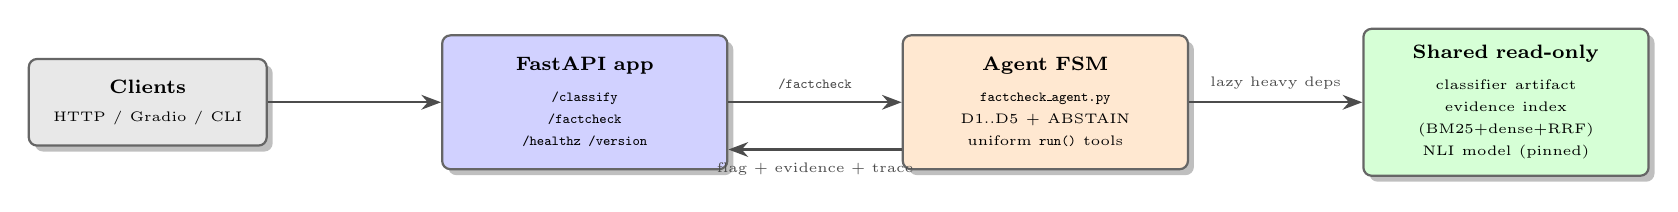
\begin{tikzpicture}[
  node distance=1.0cm and 2.2cm,
  box/.style={rectangle, draw=black!60, rounded corners=3pt, thick,
             text width=3.2cm, minimum height=1.7cm, align=center,
             inner sep=6pt, font=\scriptsize, drop shadow},
  clientbox/.style={box, fill=gray!18, text width=2.6cm, minimum height=1.1cm},
  apibox/.style={box, fill=blue!18},
  agentbox/.style={box, fill=orange!18},
  statebox/.style={box, fill=green!16},
  arrow/.style={-{Stealth[length=2.5mm]}, thick, color=black!70}
]

\node[clientbox] (cli) {\textbf{Clients}\\[2pt]{\tiny HTTP / Gradio / CLI}};
\node[apibox, right=of cli] (api) {%
  \textbf{FastAPI app}\\[3pt]
  {\tiny \texttt{/classify}}\\
  {\tiny \texttt{/factcheck}}\\
  {\tiny \texttt{/healthz} \texttt{/version}}
};
\node[agentbox, right=of api] (agent) {%
  \textbf{Agent FSM}\\[3pt]
  {\tiny \texttt{factcheck\_agent.py}}\\
  {\tiny D1..D5 + ABSTAIN}\\
  {\tiny uniform \texttt{run()} tools}
};
\node[statebox, right=of agent] (state) {%
  \textbf{Shared read-only}\\[3pt]
  {\tiny classifier artifact}\\
  {\tiny evidence index}\\
  {\tiny (BM25+dense+RRF)}\\
  {\tiny NLI model (pinned)}
};

\draw[arrow] (cli.east) -- (api.west);
\draw[arrow] (api.east) -- node[above=1pt, font=\tiny] {\texttt{/factcheck}} (agent.west);
\draw[arrow] (agent.east) -- node[above=1pt, font=\tiny] {lazy heavy deps} (state.west);
\draw[arrow] ([yshift=-6mm]agent.west) -- node[below=1pt, font=\tiny] {flag + evidence + trace} ([yshift=-6mm]api.east);

\end{tikzpicture}%
}
\caption{Single-app, two-signal deployment architecture. The cheap classifier prior runs per request; the heavier retrieval+NLI fact-check (the agent FSM) is gated behind \texttt{/factcheck}. Heavy imports happen inside each tool's \texttt{run()} and degrade gracefully -- with no torch the service still boots on the TF-IDF + BM25 path.}
\label{fig:arch}
\end{figure}

\subsection{Endpoints}

\begin{table}[H]
\centering
\caption{FastAPI endpoints}
\small
\begin{tabularx}{\linewidth}{@{} l l L @{}}
\toprule
\textbf{Endpoint} & \textbf{Method} & \textbf{Request / response} \\
\midrule
\texttt{/classify} & POST & \texttt{\{text\}} or \texttt{\{title, body\}} $\rightarrow$ \texttt{\{label, probability, prior\_fake, model\_version, backend\}} \\
\texttt{/factcheck} & POST & \texttt{\{claim, k?, threshold?\}} $\rightarrow$ \texttt{\{verdict, confidence, classifier\_prior, evidence[\{text,source,stance,score\}], rationale, decisions\_trace, disclaimer, abstained\}} \\
\texttt{/healthz} & GET & \texttt{\{status, models\_loaded\}} (503 until index/model warm) \\
\texttt{/version} & GET & \texttt{\{api, classifier\_version, nli\_model, retriever, index\_built\_at, git\_sha\}} \\
\bottomrule
\end{tabularx}
\end{table}

\noindent \texttt{/classify} returns the calibrated probability of the \emph{fake} class as an explicit \emph{prior}, not a verdict. \texttt{/factcheck} runs the FSM and \textbf{always} returns the evidence list, a \texttt{disclaimer} and the \texttt{decisions\_trace} -- even on abstain -- because transparency is non-optional. The classifier prior and the evidence verdict are two separate fields so a reviewer sees a \texttt{conflict} when they disagree.

\subsection{Latency, Scaling \& Versioning}

The classifier path is fast (TF-IDF+LogReg sub-ms CPU; transformer $\sim$10--30\,ms GPU / $\sim$100--300\,ms CPU per doc) and runs per request. The retrieval+NLI fact-check is heavier ($\approx$0.3--2\,s) and is gated behind \texttt{/factcheck}, cached by claim hash, with the evidence index built offline (sparse+dense), versioned and memory-mapped. Scaling: stateless API replicas behind a load balancer share a read-only index volume; under load the gated NLI path degrades to \texttt{"unverified -- capacity"} rather than timing out. Every response (and \texttt{/version}) stamps semantic model versions and \textbf{pinned HF revisions/commit SHAs} + \texttt{index\_built\_at} so a Hub update can never silently change a verdict.

% ============================================================
\section{Agentic AI Component}
% ============================================================

\subsection{Agent Architecture}

The agentic fact-check is a \textbf{deterministic finite-state machine} with uniform \texttt{run(**kwargs)->\{ok,data,meta\}} tools and a \texttt{ToolTrace} on every transition. An \emph{optional} LLM brain (\texttt{anthropic}, opt-in, validated) may only \textbf{propose} a value from the legal set at each decision point and \textbf{never decides flow, invents a verdict, or invents a citation}; on JSON-parse-fail / out-of-set / timeout, the deterministic rule fires. States: \textsc{Ingest/Normalize} $\rightarrow$ \textsc{Parse/Claim-Extract} $\rightarrow$ \textsc{Classify} $\rightarrow$ \textsc{Check-Worthy?} $\rightarrow$ \textsc{Retrieve} $\rightarrow$ \textsc{Stance/NLI} $\rightarrow$ \textsc{Aggregate} $\rightarrow$ \textsc{Decide/Abstain} $\rightarrow$ \textsc{Present}, with \textsc{Abstain} reachable from any state.

\begin{figure}[H]
\centering
\resizebox{\linewidth}{!}{%
\begin{tikzpicture}[
  node distance=0.30cm,
  step/.style={rectangle, draw=black!60, rounded corners=2pt, thick,
              text width=13.5cm, inner sep=5pt, minimum height=0.7cm,
              align=center, font=\footnotesize},
  in/.style={step, fill=gray!15},
  clf/.style={step, fill=purple!15},
  dec/.style={step, fill=red!12},
  ir/.style={step, fill=blue!15},
  nli/.style={step, fill=orange!15},
  abst/.style={step, fill=yellow!22},
  pres/.style={step, fill=green!15},
  arrow/.style={-{Stealth[length=2mm]}, thick}
]

\node[in] (a0) {\textbf{Ingest / Parse}: normalise input; classify \texttt{doc\_type} (article vs short claim)};
\node[dec, below=of a0] (a1) {\textbf{D1 -- Claim routing}: \texttt{len(tokens)$\leq$40} or no body $\rightarrow$ short-claim; else article $\rightarrow$ extract central claim (title / lead / TextRank)};
\node[clf, below=of a1] (a2) {\textbf{Classify} (\textit{tool}): transformer / TF-IDF $\rightarrow$ prior $P(\text{fake})$, \texttt{backend}};
\node[dec, below=of a2] (a3) {\textbf{D2 -- Check-worthiness gate}: skip retrieval iff \texttt{conf$\geq\tau_{\text{skip}}{=}0.95$} AND \texttt{checkworthy$<\tau_{\text{cw}}{=}0.5$} (confident non-claim $\rightarrow$ present prior)};
\node[ir, below=of a3] (a4) {\textbf{Retrieve} (\textit{tool}): BM25 + dense (\texttt{all-MiniLM-L6-v2}) $\rightarrow$ RRF $\rightarrow$ rerank};
\node[dec, below=of a4] (a5) {\textbf{D3 -- Evidence-coverage gate}: keep \texttt{rerank$\geq\tau_{\text{rel}}$}; OK iff \texttt{$n_{\text{rel}}\geq N_{\min}{=}3$}; else widen $\leq R_{\max}{=}2$ then \textbf{ABSTAIN}};
\node[nli, below=of a5] (a6) {\textbf{Stance / NLI} (\textit{tool}): per evidence, premise=evidence, hypothesis=claim $\rightarrow$ support / refute / neutral};
\node[dec, below=of a6] (a7) {\textbf{D4 -- Verdict gate}: $S=\sum w_i s_i$; combine prior at $\alpha{=}0.6$; $|S|{>}\theta{=}0.2 \rightarrow$ REAL / FAKE else \textbf{UNVERIFIED}};
\node[dec, below=of a7] (a8) {\textbf{D5 -- Confidence / abstain gate}: abstain if UNVERIFIED, low agreement ($<\tau_{\text{agree}}{=}0.4$), low conf ($<\tau_{\text{present}}{=}0.55$), or prior$\leftrightarrow$stance \texttt{conflict}};
\node[pres, below=of a8] (a9) {\textbf{Present}: label + confidence + \textbf{verbatim citations} + rationale + \texttt{decisions\_trace}\quad(or ``\texttt{unverified} -- needs human review'')};

\foreach \a/\b in {a0/a1, a1/a2, a2/a3, a3/a4, a4/a5, a5/a6, a6/a7, a7/a8, a8/a9}
  \draw[arrow] (\a) -- (\b);

\end{tikzpicture}%
}
\caption{The agent FSM with five explicit decision points D1--D5. Each decision acts on the model's own intermediate outputs; ABSTAIN is reachable from D3 and D5. The brain (optional) only proposes legal values -- the deterministic rule always governs flow.}
\label{fig:agent}
\end{figure}

\subsection{Decision Table (the $\geq 5$ decision points)}

\begin{table}[H]
\centering
\caption{The five FSM decision points (each acts on intermediate outputs)}
\small
\begin{tabularx}{\linewidth}{@{} l l L L @{}}
\toprule
\textbf{ID} & \textbf{State} & \textbf{Rule / threshold} & \textbf{Branches} \\
\midrule
\textbf{D1} & Parse / Claim-extract & \texttt{len(tokens)$\leq$40} OR no body $\rightarrow$ short-claim; else article (central claim = title / lead / TextRank); \texttt{claim\_len$\geq$5} else \texttt{INVALID\_INPUT} & short claim \quad/\quad article \\
\textbf{D2} & Check-worthiness & skip gate = (\texttt{conf$\geq\tau_{\text{skip}}{=}0.95$}) AND (\texttt{checkworthy$<\tau_{\text{cw}}{=}0.5$}); \texttt{checkworthy} = entity/number/verifiable-predicate heuristic & skip $\rightarrow$ present prior \quad/\quad proceed $\rightarrow$ retrieve \\
\textbf{D3} & Retrieve (coverage) & after RRF, keep \texttt{rerank$\geq\tau_{\text{rel}}$}; coverage OK iff \texttt{$n_{\text{rel}}\geq N_{\min}{=}3$}; else widen $\leq R_{\max}{=}2$ then abstain & enough $\rightarrow$ stance \quad/\quad thin $\rightarrow$ widen \quad/\quad exhausted $\rightarrow$ ABSTAIN \\
\textbf{D4} & Aggregate (verdict) & per-evidence: entail $+1$, contra $-1$, neutral $0$, weighted by relevance; \texttt{score $= \alpha\cdot$stance $+ (1{-}\alpha)\cdot$prior}, $\alpha{=}0.6$; verdict by $\theta{=}0.2$ & REAL \quad/\quad FAKE \quad/\quad UNVERIFIED \\
\textbf{D5} & Decide / Abstain & abstain if UNVERIFIED, \texttt{agreement$<\tau_{\text{agree}}{=}0.4$}, \texttt{final\_conf$<\tau_{\text{present}}{=}0.55$}, or prior$\leftrightarrow$stance conflict & present \quad/\quad abstain (``needs human review'') \\
\bottomrule
\end{tabularx}
\end{table}

\noindent \textbf{Evidence dominates; the classifier prior is a soft nudge.} The decision rules satisfy all rubric requirements for an agent: \emph{multi-step reasoning} (D1, D3, D4), \emph{tool usage} (classify, retrieve, stance), and \emph{decision-making on intermediate outputs} (D2, D5).

\subsection{Example Trace (every decision fires)}

\begin{lstlisting}
# Input (short claim):
"The WHO declared that drinking bleach cures COVID-19 in 2021."

1) Ingest/Parse  -> doc_type="claim", short body
   Classify      -> label="fake", p_fake=0.88, backend="transformer"
2) D1 ClaimExtract -> 11 tokens <= 40 -> short-claim route
   claim = input; entities=["WHO","COVID-19","2021","bleach"]; method=title
3) D2 CheckWorthy  -> conf 0.88 < tau_skip 0.95 -> do NOT skip
   checkworthy=0.92 (named org + medical predicate + date) -> RETRIEVE
4) D3 Retrieve     -> RRF(BM25,dense) -> 4 passages with rerank >= 0.3
   n_relevant=4 >= N_min=3 -> coverage_ok, no widen
5) Stance/NLI      -> 3x contradiction->refute (~0.94), 1x neutral
6) D4 Aggregate    -> S = -(0.94+0.91+0.88) ~ -2.7; prior agrees
   |S| > theta=0.2 -> verdict=FAKE/REFUTED, n_refute=3, conf=0.91
7) D5 Decide       -> agreement |0-3|/4 = 0.75 >= 0.4; conf 0.91 >= 0.55
   prior agrees (no conflict) -> action=present
8) Present         -> label="fake", confidence=0.91,
   citations=[3 refuting WHO/fact-check passages: id+source+snippet+stance],
   rationale="Multiple authoritative sources contradict this claim;
              no source supports it.", abstained=false, ToolTrace attached

# Counter-example (abstain):
A novel claim with no corpus coverage -> D3 widens twice, still n_relevant<3
   -> ABSTAIN "unverified (insufficient evidence)" -- never a guessed label
\end{lstlisting}

% ============================================================
\section{Continual Learning \& Monitoring}
% ============================================================

\subsection{Monitoring Strategy}

\begin{itemize}\setlength\itemsep{0.15em}
  \item \textbf{Prediction logging}: each request logged to JSONL with the classifier prior, the evidence verdict, the action (present/abstain), the backend used, and the model versions from \texttt{/version}.
  \item \textbf{Drift detection} (\texttt{monitoring/drift\_report.py}): monitors input-text drift and label/verdict-rate drift over time -- a shift in abstain rate or in the prior$\leftrightarrow$verdict conflict rate is an early signal.
  \item \textbf{Error slices} (\texttt{analysis/error\_analysis.py}, \texttt{fairness.py}): errors are sliced per-source/outlet, per-topic (politics/health/science/finance) and per-speaker (LIAR) rather than reported as one aggregate, to expose bias and leakage.
\end{itemize}

\subsection{Continual Learning Strategy}

\begin{enumerate}\setlength\itemsep{0.15em}
  \item Collect borderline cases and reviewer overrides from the human-review queue (the flag-for-review feedback loop).
  \item Re-label with documented provenance; record reviewer ``was the evidence useful?'' signals as a flag-queue precision metric.
  \item Retrain the classifier on old + new data; re-fit temperature scaling on a fresh calibration split; rebuild and re-version the evidence index.
  \item Re-evaluate on test + the \textbf{cross-domain} split + fairness slices (the leakage audit is a periodic gate).
  \item Deploy with versioning (pinned revisions) so a champion/challenger rollout and per-model rollback are trivial; the model registry is the integration ledger.
\end{enumerate}

% ============================================================
\section{Data Privacy \& Model Robustness}
% ============================================================

\subsection{Privacy}

\begin{itemize}
  \item Citations are extracted \textbf{verbatim} from the retrieved corpus with source ids -- never generated -- so a fact-check is auditable and never misattributes a source.
  \item No hard-coded credentials; secrets via environment variables; the optional LLM brain is opt-in.
  \item Logging records the classifier/verdict signals and version stamps for monitoring, not enforcement actions.
\end{itemize}

\subsection{Robustness}

\begin{itemize}\setlength\itemsep{0.15em}
  \item \textbf{Source-style leakage}: measured via the cross-domain drop; the trusted output is the \emph{evidence verdict}, not the style prior.
  \item \textbf{Adversarial paraphrase / evasion}: bad actors paraphrase to flip a \emph{style} classifier -- the evidence-grounded fact-check is more robust; no ``evasion score'' is shipped (dual-use).
  \item \textbf{Stale / out-of-scope evidence}: the index is versioned and timestamped (\texttt{/version}); D3 abstains when retrieval coverage is thin rather than fabricating evidence.
  \item \textbf{No-torch degradation}: with heavy libs absent the classifier falls back to TF-IDF+LogReg, the retriever to BM25, and stance to a lexical mock -- the API contract \emph{never} breaks.
\end{itemize}

% ============================================================
\section{Project Management}
% ============================================================

This project was completed \emph{individually}, but planned as if delivered by a simulated cross-functional team (PM, classifier MLE, IR engineer, NLI engineer, backend, MLOps, and a dedicated \textbf{Ethics/Safety reviewer} with sign-off authority at three gates).

\begin{table}[H]
\centering
\caption{Project timeline (milestones; each has a CPU/offline acceptance gate before the GPU path)}
\small
\begin{tabularx}{\linewidth}{@{} l l L @{}}
\toprule
\textbf{Milestone} & \textbf{Wk} & \textbf{Exit / acceptance gate} \\
\midrule
M0 Design locked & 1 & \texttt{DESIGN\_BRIEF.md} signed off; all HF ids + licenses + polarity verified \\
M1 Offline skeleton & 2 & Full pipeline on \texttt{samples.py} with no torch / no network \\
M2 Data + baseline & 3 & All loaders apply per-source \texttt{label\_map}; TF-IDF baseline macro-F1 logged \\
M3 Classifier + calibration & 4 & Transformer trained; ECE pre/post; boilerplate stripped \\
M4 Evidence retriever & 5 & recall@k vs \texttt{BeIR/fever-qrels}; BM25 fallback works (ETH: corpus license gate) \\
M5 Stance + verdict + FSM & 6 & Worked + abstain examples reproduce; D1--D5 traced (ETH: abstain is first-class) \\
M6 API / UI / CLI / Docker & 7 & Service boots on core-only install; \texttt{/factcheck} always returns evidence + trace \\
M7 Evaluation + cross-domain & 8 & In-domain \textbf{and} cross-domain tables (ETH: drop reported honestly) \\
M8 Report / slides / grade & 9 & \texttt{autopilot} green; \texttt{grade} passes; ETH final no-censorship sign-off \\
\bottomrule
\end{tabularx}
\end{table}

\textbf{Critical path}: M1$\rightarrow$M2$\rightarrow$M3$\rightarrow$M5$\rightarrow$M7$\rightarrow$M8; the retriever (M4) runs in parallel with the classifier (M3). The single longest pole is \emph{data normalisation + leakage control}, the fake-news-specific trap -- not the modelling. The uniform tool contract and typed \texttt{AppConfig} are the only shared interfaces, so the seven simulated roles map 1:1 to modules and scale to seven real people with minimal rework.

% ============================================================
\section{Ethics \& Responsible AI}
% ============================================================

This is the most ethically loaded project in the set, and the design treats ethics as a first-class workstream. \textbf{The system flags content for human review; it never auto-removes, auto-blocks, or auto-censors, and it always shows its evidence.} It assists human fact-checkers; it is not an automated arbiter of truth.

\subsection{Who Benefits}

Fact-checkers and moderators (a better-triaged queue, less time on clearly-credible items), newsrooms (an auditable credibility signal), and readers (transparency that encourages verification rather than blind trust).

\subsection{Who Could Be Harmed, and the Mitigations}

\begin{table}[H]
\centering
\caption{Key risks and concrete mitigations (baked into the deliverable)}
\small
\begin{tabularx}{\linewidth}{@{} L L @{}}
\toprule
\textbf{Risk} & \textbf{Mitigation} \\
\midrule
Censorship / free-speech chilling & Output is a \textbf{review flag + evidence}, never an enforcement action; no auto-takedown anywhere; verdicts are advisory \\
False positives silencing real news (the high-cost error) & Optimise the operating point for high \texttt{real}-recall; report per-class costs; \textbf{abstain} rather than guess; human sign-off before any action \\
Political bias in labels/data & Document label provenance; report performance sliced by topic/speaker/source; never present output as neutral ground truth \\
Source-style leakage & Measure the cross-domain drop; strip/ablate style features; trust the \emph{evidence} verdict; treat the prior as a weak signal only \\
Automation bias / over-trust & Calibration (ECE) + mandatory confidence display; abstain on uncertainty; UI states it is decision-support requiring the evidence to be read \\
Hallucinated / misattributed citations & Citations extracted \textbf{verbatim} with source ids, never generated; \texttt{decisions\_trace} lets a reviewer verify each one \\
Dual-use (evasion crafting) & No ``evasion score'' shipped; rate-limit; log; gate adversarial tooling \\
Stale / out-of-scope evidence & Version + timestamp the index; \textbf{abstain} when coverage is insufficient rather than fabricate \\
\bottomrule
\end{tabularx}
\end{table}

\subsection{Limitations Stated Plainly}

English-centric data; PolitiFact/GossipCop domain skew (US politics + celebrity); ``fake/real'' is a coarse proxy for a spectrum (LIAR's 6-way captures this better); the system verifies against a \emph{fixed corpus} and cannot know facts outside it. \textbf{\texttt{unverified} means \emph{insufficient evidence}, not \emph{true}.} The classifier detects \emph{style/source patterns correlated with fakeness}, which is not detecting falsehood -- the agentic evidence layer compensates, and \texttt{classifier\_prior} vs.\ evidence \texttt{verdict} are reported \textbf{separately} so a reviewer sees disagreement. \textbf{Design commitments baked in}: mandatory transparency + verbatim citations on every verdict; abstain under uncertainty as a first-class outcome; assist rather than replace human judgement; never take an irreversible action on content automatically.

% ============================================================
\section{Conclusion}
% ============================================================

This project delivers a complete, honest, end-to-end fake-news detection system: a trainable transformer classifier (with majority/TF-IDF/zero-shot baselines) for a fast credibility prior, wrapped by a deterministic five-decision agent FSM that retrieves evidence, judges stance, aggregates an evidence-grounded verdict with verbatim citations, and \textbf{abstains} when uncertain. The verified offline seed run proves the full metric and FSM plumbing with no torch (classifier acc/macro-F1/ROC-AUC = 1.0 on an engineered-separable seed, ECE = 0.244 demonstrating the over-confidence pathology; fact-check label accuracy = 1.0, coverage = 1.0 with abstain reachable), while the Colab H100 autopilot produces the full-scale numbers -- including the cross-domain drop that is the honest classifier metric. The deliverable is deployable across REST API, Gradio UI, CLI and Docker/Space, and is built on a single non-negotiable principle: \emph{it flags for human review, never censors, and always shows its evidence.}

\textbf{Future work}: active learning from the human-review queue; a FEVER-fine-tuned stance head (with share-alike attribution); larger backbones (ModernBERT-large) and more languages; token-level explainability; and a drift dashboard with champion/challenger A/B testing.

\end{document}
